% =====================================================================
%  Legendre's Conjecture in Function Fields:
%  Full Monodromy, Twisted Root Varieties, and Explicit Bounds
%  Version v6, DOI 10.5281/zenodo.23179113 (revises v5, DOI 10.5281/zenodo.18705744)
% =====================================================================
\documentclass[11pt,a4paper]{article}

\usepackage[top=28mm,bottom=28mm,left=25mm,right=25mm]{geometry}
\usepackage[T1]{fontenc}
\usepackage{lmodern}
\usepackage{amsmath,amssymb,amsthm,mathtools}
\usepackage{graphicx}
\usepackage{booktabs}
\usepackage[dvipsnames]{xcolor}
\usepackage{enumitem}
\usepackage[colorlinks=true,linkcolor=MidnightBlue,citecolor=MidnightBlue,urlcolor=MidnightBlue]{hyperref}

\newtheorem{theorem}{Theorem}[section]
\newtheorem{lemma}[theorem]{Lemma}
\newtheorem{proposition}[theorem]{Proposition}
\newtheorem{corollary}[theorem]{Corollary}
\newtheorem*{theoremA}{Theorem A}
\newtheorem*{theoremB}{Theorem B}
\newtheorem*{theoremC}{Theorem C}
\newtheorem*{theoremD}{Theorem D}
\theoremstyle{definition}
\newtheorem{definition}[theorem]{Definition}
\newtheorem{example}[theorem]{Example}
\theoremstyle{remark}
\newtheorem{remark}[theorem]{Remark}

\newcommand{\Fq}{\mathbb{F}_q}
\newcommand{\Fqbar}{\overline{\mathbb{F}}_q}
\newcommand{\A}{\mathbb{A}}
\newcommand{\Gal}{\mathrm{Gal}}
\newcommand{\Tr}{\mathrm{Tr}}
\newcommand{\disc}{\mathrm{disc}}
\newcommand{\Ggeom}{G_{\mathrm{geom}}}
\newcommand{\Nirr}{N_{\mathrm{irr}}}
\newcommand{\cI}{\mathcal{I}}
\newcommand{\cM}{\mathcal{M}}
\newcommand{\cH}{\mathcal{H}}
\newcommand{\ba}{\mathbf{a}}

\title{\textbf{Legendre's Conjecture in Function Fields:\\
Full Monodromy, Twisted Root Varieties,\\ and Explicit Bounds}\\[4pt]
\large Revised version (v6) of \textit{The Geometry of Prime Vacuums}}
\author{Ruqing Chen\\[3pt]
\small GUT Geoservice Inc., Montr\'eal, Canada\\
\small \texttt{ruqing@hotmail.com}}
\date{October 2026\\[2pt]\small DOI: \href{https://doi.org/10.5281/zenodo.23179113}{10.5281/zenodo.23179113}\quad Code and data: \url{https://github.com/Ruqing1963/legendre-function-field}}

\begin{document}
\maketitle

\begin{abstract}
For a monic polynomial $f\in\Fq[t]$ of degree $d\ge1$, the
\emph{Legendre interval} $\cI_f=\{f^2+s:\ \deg s\le d\}$ is the natural
function field analogue of $[n^2,(n+1)^2]$.
That $\cI_f$ contains $q^{d+1}/(2d)+O_d(q^{d+1/2})$ irreducible polynomials
is a special case ($\epsilon=1/2$) of the short-interval theorem of
Bank, Bary-Soroker and Rosenzweig (2015); the earlier version (v5) of
this preprint presented it as new, and this revision corrects that.
We give a self-contained proof that the geometric monodromy group of the
family is the full symmetric group $S_{2d}$ whenever $p=\mathrm{char}\,\Fq>2d$,
\emph{without} the squarefree hypothesis on $f$ that v5 required.
We then prove an exact identity
$2d\,\Nirr=\#W(\Fq)-E$, where $W$ is an explicit
$(d+1)$-dimensional twisted form of the root variety of the family,
of degree at most $(d-1)!$, and $0\le E<q^{d+1}/(q-1)$.
Combined with the explicit Lang--Weil estimate of Cafure and Matera,
this yields a fully explicit and rigorous threshold
$q_0(d)$ beyond which every Legendre interval contains an irreducible polynomial.
For $d\le 3$ we obtain closed formulas valid for every admissible $q$;
for $d=3$ they agree with Kuz'min's count of irreducible polynomials with
two prescribed coefficients.
Exhaustive and sampled computations for $d\le6$ support every statement,
and the code and data are public.
An appendix lists the errors in v5 and how each one is fixed here.
\end{abstract}

\tableofcontents
\bigskip

% =====================================================================
\section{Introduction}\label{sec:intro}
% =====================================================================

\subsection{Background}
Legendre's conjecture asserts that for every integer $n\ge1$ there is a
prime between $n^2$ and $(n+1)^2$. It is open; the best unconditional result
on prime gaps (Baker--Harman--Pintz \cite{BHP2001}) gives primes in
$[x,x+x^{0.525}]$, whereas the Legendre interval has length about $2x^{1/2}$.

In $\Fq[t]$ the absolute value is $|g|=q^{\deg g}$. For monic $f$ of degree
$d$ the polynomials $g$ with $|g-f^2|\le|f|$ are exactly
\[
  \cI_f=\{\,f^2+s:\ s\in\Fq[t],\ \deg s\le d\,\},\qquad |\cI_f|=q^{d+1},
\]
an interval of ``length'' $|f|=|f^2|^{1/2}$ around $f^2$, the analogue of
$[n^2,n^2+n]\subset[n^2,(n+1)^2]$. All elements of $\cI_f$ are monic of degree $2d$.
The prime polynomial theorem predicts about $|\cI_f|/(2d)$ irreducibles.

\begin{definition}\label{def:interval}
Write $\cM=\A^{d+1}$ with coordinates $\ba=(a_0,\dots,a_d)$ and put
\[
  F(t,\ba)=f(t)^2+\sum_{i=0}^{d}a_it^i,\qquad
  \Nirr(f)=\#\{\ba\in\Fq^{d+1}:\ F(t,\ba)\ \text{irreducible in}\ \Fq[t]\}.
\]
\end{definition}

\subsection{What was already known}
Bank, Bary-Soroker and Rosenzweig \cite{BBR2015} proved that for every
partition $\lambda$ of $k$, every monic $f$ of degree $k$ and every $m$ with
$1\le m<k$ (with $m\ge2$ if $p\mid k(k-1)$, and $m\ge 3$ if $p=2$ and
$\deg f'\le 1$), the number of $g\in f+\Fq[t]_{\le m}$ with factorization type
$\lambda$ is $P(\lambda)q^{m+1}+O_k(q^{m+1/2})$, where $P(\lambda)$ is the
proportion of permutations of cycle type $\lambda$ in $S_k$.
Taking $k=2d$, $m=d$ and replacing $f$ by $f^2$ gives, for every odd $q$,
\begin{equation}\label{eq:BBR}
  \Nirr(f)=\frac{q^{d+1}}{2d}+O_d\bigl(q^{d+1/2}\bigr).
\end{equation}
This is exactly the ``Main Theorem'' of v5 of this preprint, which therefore
is not new. The implied constant in \cite{BBR2015} is not explicit.

\subsection{Results of this paper}
Throughout, $q$ is a power of a prime $p$, and $f\in\Fq[t]$ is monic of degree $d\ge1$.
We write $\Ggeom$ for the Galois group of $F(t,\ba)$ over $\Fqbar(\ba)$,
i.e.\ the geometric monodromy group of the finite cover
$\{F=0\}\to\cM$ (Section~\ref{sec:monodromy}).

\begin{theoremA}[Section~\ref{sec:monodromy}]
If $p>2d$, then $\Ggeom=S_{2d}$. No assumption on $f$ beyond monicity is needed.
\end{theoremA}

\begin{theoremB}[Section~\ref{sec:twisted}]
There is an affine variety $W$ over $\Fq$, explicitly defined by $d-1$
equations of degrees $1,2,\dots,d-1$ in $\A^{2d}$, such that for all $q$
\[
  2d\cdot\Nirr(f)=\#W(\Fq)-E(f),\qquad 0\le E(f)\le\sum_{e\mid 2d,\ e<2d}q^e<\frac{q^{d+1}}{q-1}.
\]
Its $\Fq$-points are the $\beta\in\mathbb{F}_{q^{2d}}$ whose characteristic polynomial lies in $\cI_f$.
$W$ has pure dimension $d+1$ and degree at most $(d-1)!$, and it is
absolutely irreducible if and only if $\Ggeom=S_{2d}$.
\end{theoremB}

\begin{theoremC}[Section~\ref{sec:explicit}]
Assume $\Ggeom=S_{2d}$ (for instance $p>2d$). Let $\delta=(d-1)!$. If $q>2(d+2)\delta^2$, then
\[
  \bigl|\,2d\,\Nirr(f)-q^{d+1}\bigr|
  <(\delta-1)(\delta-2)\,q^{d+1/2}+\bigl(5\delta^{13/3}+2\bigr)q^{d}.
\]
Consequently $\Nirr(f)\ge1$ for all $q>q_0(d):=\max\bigl\{2(d+2)\delta^2,\ \bigl((\delta-1)(\delta-2)+\sqrt{5\delta^{13/3}+2}\bigr)^2\bigr\}$.
\end{theoremC}

\begin{theoremD}[Section~\ref{sec:small}]
(i) If $d=1$ then $\Nirr=(q^2-q)/2$.
(ii) If $d=2$ and $q$ is odd then $\Nirr=(q^3-q)/4$.
(iii) If $d=3$ and $p\ge5$, write $f=t^3+c_2t^2+c_1t+c_0$ and $\Delta=c_2^2-3c_1$; let $\eta$
be the quadratic character of $\Fq$. Then
\[
 6\,\Nirr=\begin{cases}
 q^4-\eta(2\Delta)\,q^2-q+\eta(-3)+\eta(2\Delta)-1, & \Delta\ne0,\\[2pt]
 q^4-q-(q-1)\,\eta(-3), & \Delta=0.
 \end{cases}
\]
In particular every Legendre interval with $d\le3$ contains an irreducible
polynomial, for every $q$ in the stated range.
\end{theoremD}

Theorem~C gives, for example, $q_0(4)\approx1.65\times10^{4}$ and
$q_0(5)\approx7.3\times10^{6}$ (Table~\ref{tab:thresholds}).
For $d\le3$ no threshold is needed.
Theorem~D(i)--(ii) are classical consequences of the counts of irreducible
polynomials with prescribed trace \cite{Carlitz1952}, and (iii) is a special
case of Kuz'min's formula for two prescribed coefficients
(see \cite{LL2016,MY2016}). We include short proofs because they come out of
Theorem~B directly and they make good test cases for the computations.

The genuinely hard analogue of Legendre's conjecture fixes $q$ and lets
$d\to\infty$. Then one must prescribe the top $d-1$ coefficients of a
polynomial of degree $2d$, about half of them.
Existing results on irreducible polynomials with prescribed coefficients
\cite{Pollack2013,Ha2016} handle far fewer coefficients, so this regime
remains open (Section~\ref{sec:discussion}).

\subsection{About this revision}
Version v5 \cite{ChenV5} contained several gaps and incorrect citations,
listed in Appendix~\ref{app:errata}. The most serious were:
the main theorem was not new; the primitivity argument used a criterion that
does not apply as stated; the effective Chebotarev bound was formulated with
the wrong sheaf; and the explicit threshold $(8d)^{2d+6}$ relied on a
Betti-number estimate that is not in the cited source.
The present version replaces the cohomological error analysis by the
elementary twisted-variety identity (Theorem~B) and an explicit Lang--Weil
bound, so that every constant is proved.

% =====================================================================
\section{Preliminaries}\label{sec:prelim}
% =====================================================================

For $\beta\in\mathbb{F}_{q^{n}}$ let
$\chi_\beta(t)=\prod_{k=0}^{n-1}(t-\beta^{q^k})\in\Fq[t]$ be its
characteristic polynomial over $\Fq$. If $\beta$ has degree $e\mid n$ over $\Fq$
and minimal polynomial $\mu_\beta$, then $\chi_\beta=\mu_\beta^{\,n/e}$.

\begin{lemma}[Membership in $\cI_f$]\label{lem:membership}
A monic $P\in\Fq[t]$ of degree $2d$ lies in $\cI_f$ if and only if its
coefficients of $t^{2d-1},\dots,t^{d+1}$ agree with those of $f^2$.
If $p>d-1$, this holds if and only if the power sums
$p_j(P)=\sum_{P(\rho)=0}\rho^j$ satisfy $p_j(P)=2\,p_j(f)$ for $1\le j\le d-1$.
\end{lemma}

\begin{proof}
The first statement is the definition. For the second, Newton's identities
express the power sums $p_1,\dots,p_{d-1}$ through the top $d-1$ coefficients.
The converse direction needs division by $1,\dots,d-1$, which is allowed when $p>d-1$.
Finally $p_j(f^2)=2p_j(f)$.
\end{proof}

\begin{lemma}[Inertia at a simple node]\label{lem:node}
Let $R$ be a complete discrete valuation ring with algebraically closed residue
field $k$ of characteristic $\ne2$, fraction field $K$ and valuation $v$.
Let $P\in R[t]$ be monic of degree $n$ whose reduction $\bar P$ has exactly
one double root $\beta$ and $n-2$ simple roots, and suppose $v(\disc P)=1$.
Then the splitting field of $P$ over $K$ is a quadratic extension whose
Galois group acts on the roots of $P$ as a transposition.
\end{lemma}

\begin{proof}
Write $\bar P=(t-\beta)^2\bar L$ with $\bar L(\beta)\neq0$ and $\bar L$ squarefree.
By Hensel's lemma $P=QL$ with $Q,L\in R[t]$ monic lifting $(t-\beta)^2$ and $\bar L$,
and $L$ splits into linear factors over $R$.
Since $\disc P=\disc Q\cdot\disc L\cdot\mathrm{Res}(Q,L)^2$ and both
$\disc L$ and $\mathrm{Res}(Q,L)$ are units, $v(\disc Q)=1$.
An element of odd valuation is not a square in $K$, so $Q$ is irreducible over
$K$ and its splitting field is a quadratic extension. Its nontrivial automorphism
swaps the two roots of $Q$ and fixes the roots of $L$.
\end{proof}

\begin{lemma}[Primitivity and decomposition; cf.\ \cite{Turnwald1995,Muller1995}]\label{lem:luroth}
Let $K$ be a field, $G\in K[t]$ of degree $n\ge2$ with $G'\neq0$, and $x$
transcendental over $K$. If $\Gal(G(t)-x\,/\,K(x))$, acting on the roots of $G(t)-x$,
is imprimitive, then $G=g\circ h$ with $g,h\in K[t]$ and $\deg g,\deg h\ge2$.
\end{lemma}

\begin{proof}
Let $\tau$ be a root and $\Gamma$ the Galois group. Blocks containing $\tau$
correspond to subgroups between the stabilizer of $\tau$ and $\Gamma$, hence
to fields $K(x)\subseteq L\subseteq K(\tau)$. Imprimitivity gives a proper
intermediate field $L$, and $L=K(h)$ for some $h\in K(\tau)$ by L\"uroth's theorem.
Since $x=G(\tau)$ is a polynomial in $\tau$, the place $\tau=\infty$ is the only
place of $K(\tau)$ above $x=\infty$; it is $K$-rational. Its restriction to $L$ is
therefore the only place of $L$ above $x=\infty$, and it is $K$-rational.
After a M\"obius transformation over $K$ we may take it to be $h=\infty$.
Then $h$, as a function of $\tau$, has its only pole at $\tau=\infty$, so $h\in K[\tau]$.
Likewise $x\in K(h)$ has its only pole at $h=\infty$, so $x=g(h)$ with $g\in K[X]$.
Both degrees are $\ge2$ because $L$ is a proper intermediate field.
\end{proof}

% =====================================================================
\section{The monodromy group}\label{sec:monodromy}
% =====================================================================

Let $\cH=\{F(t,\ba)=0\}\subset\cM\times\A^1$ and $\pi:\cH\to\cM$ the
projection, a finite flat morphism of degree $2d$. Let
$\mathcal D\subset\cM$ be the zero locus of $\disc_t F$ and $\cM^\circ=\cM\setminus\mathcal D$.
Over $\cM^\circ$, $\pi$ is finite \'etale. Its geometric monodromy group is the
image of $\pi_1(\cM^\circ_{\Fqbar})$ in $S_{2d}$, which equals
$\Ggeom=\Gal\bigl(F\,/\,\Fqbar(\ba)\bigr)$.
Put $K'=\Fqbar(a_1,\dots,a_d)$ and
\[
  G(t)=f(t)^2+a_1t+\dots+a_dt^d\in K'[t],\qquad\text{so}\qquad F=G(t)+a_0 .
\]
Since $a_0$ is transcendental over $K'$, $\Ggeom=\Gal(G(t)-x\,/\,K'(x))$ with $x=-a_0$.

\begin{proposition}[Transitivity]\label{prop:irred}
$F$ is irreducible over $\Fqbar(\ba)$, so $\Ggeom$ is transitive.
\end{proposition}
\begin{proof}
$F$ has degree one in $a_0$ with coefficients $1$ and $f^2+\sum_{i\ge1}a_it^i$,
which are coprime. Hence $F$ is irreducible in $\Fqbar[\ba,t]$, and by Gauss's
lemma it is irreducible in $\Fqbar(\ba)[t]$ because it is monic in $t$.
\end{proof}

\begin{proposition}[Primitivity]\label{prop:primitive}
If $p>d$, then $\Ggeom$ is primitive.
\end{proposition}

\begin{proof}
For $d=1$ this is automatic since $2d=2$. Let $d\ge2$. Note $G'\ne0$ because of the
term $a_1t$. Suppose $\Ggeom$ is imprimitive. By Lemma~\ref{lem:luroth} applied over
$K'$, $G=g\circ h$ with $g,h\in K'[t]$, $\deg h=m$, $\deg g=n$, $mn=2d$ and $m,n\ge2$.
In particular $m\le d$. Replacing $h$ by $\lambda h+\mu$ and $g$ accordingly, we may
assume $h$ monic with $h(0)=0$. Write $h=t^m+h_{m-1}t^{m-1}+\dots+h_1t$.

\emph{Step 1: $h$ has constant coefficients.}
For $1\le j\le m-1$ we have $2d-j\ge 2d-m+1\ge d+1$, so the coefficient of $t^{2d-j}$
in $G$ is the corresponding coefficient of $f^2$, an element of $\Fq$.
On the other side, $g(h)=c\,h^n+(\text{terms of degree}\le 2d-m)$ with $c$ the leading
coefficient of $g$, and $c=1$ because $G$ is monic. Expanding $h^n$ gives
\[
 [t^{2d-j}]\,h^n=n\,h_{m-j}+\Phi_j(h_{m-1},\dots,h_{m-j+1}),
\]
with $\Phi_j$ a polynomial with integer coefficients. Since $2\le n\le d<p$, $n$ is
invertible in $\Fq$. Induction on $j$ shows $h_{m-1},\dots,h_1\in\Fq$, so $h\in\Fq[t]$.

\emph{Step 2: contradiction.}
Let $U=\mathrm{span}_{\Fq}\{1,h,\dots,h^n\}\subset\Fq[t]_{\le2d}$. Since
$G=\sum_k g_kh^k$ with $g_k\in K'$, we get $G\in U\otimes_{\Fq}K'$.
Let $\ell$ be any $\Fq$-linear form on $\Fq[t]_{\le 2d}$ that vanishes on $U$,
extended $K'$-linearly. Then
$0=\ell(G)=\ell(f^2)+\sum_{i=1}^{d}a_i\,\ell(t^i)$ in $K'$, and since
$a_1,\dots,a_d$ are algebraically independent, $\ell(t)=0$.
As this holds for every such $\ell$, $t\in U$. But every nonconstant element of
$U$ has degree divisible by $m\ge2$. Contradiction.
\end{proof}

\begin{proposition}[A transposition]\label{prop:transposition}
If $p>2d$, then $\Ggeom$ contains a transposition.
\end{proposition}

\begin{proof}
\emph{Step 1: a fibre with exactly one double root.}
If $d=1$, take $P^\ast=(t-\beta)^2$ for any $\beta\in\Fqbar$; it lies in
$\cI_f\otimes\Fqbar$ since $\deg\bigl((t-\beta)^2-f^2\bigr)\le1$.
Let $d\ge2$ and fix $\beta\in\Fqbar$. Divide $f^2=(t-\beta)^2Q+r$ with $\deg r\le1$;
$Q$ is monic of degree $2d-2$. For $c\in\Fqbar$ put
$R_c=Q+c$ and $P^\ast=(t-\beta)^2R_c$. Then
$P^\ast-f^2=c\,(t-\beta)^2-r$ has degree $\le2\le d$, so $P^\ast$ is a fibre of $F$
over some $\ba^\ast\in\cM(\Fqbar)$. The derivative $Q'$ has leading coefficient
$2d-2\not\equiv0\pmod p$, so $R_c$ has a repeated root only if $c=-Q(\gamma)$ for a
root $\gamma$ of $Q'$. Excluding these finitely many values and $c=-Q(\beta)$,
the polynomial $R_c$ is squarefree and $R_c(\beta)\ne0$.
So $P^\ast=(t-\beta)^2R$ with $R$ squarefree and $R(\beta)\neq0$ (with $R=1$ if $d=1$).

\emph{Step 2: the discriminant vanishes to order one.}
Consider the line $\varepsilon\mapsto\ba^\ast+\varepsilon e_0$, along which
$F=P^\ast+\varepsilon$. Since $\partial_tF=P^{\ast\prime}$ does not depend on $\varepsilon$
and has leading coefficient $2d\ne0$ in $\Fq$, we have
\[
 \disc_t(P^\ast+\varepsilon)=u\prod_{\gamma:\,P^{\ast\prime}(\gamma)=0}\bigl(P^\ast(\gamma)+\varepsilon\bigr),
\]
with $u\in\Fqbar^\times$ and roots $\gamma$ counted with multiplicity. Its order of vanishing at
$\varepsilon=0$ is the number of common roots of $P^\ast$ and $P^{\ast\prime}$, counted
with their multiplicity in $P^{\ast\prime}$. Now
$P^{\ast\prime}=(t-\beta)\bigl(2R+(t-\beta)R'\bigr)$. The root $\beta$ is simple in
$P^{\ast\prime}$ because $2R(\beta)\ne0$. A root $\rho$ of $R$ is not a root of
$P^{\ast\prime}$, because $P^{\ast\prime}(\rho)=(\rho-\beta)^2R'(\rho)\ne0$.
Hence the order is exactly $1$. In particular the line is not contained in $\mathcal D$.

\emph{Step 3: inertia.}
The Galois group of $F$ restricted to the line is a subgroup of $\Ggeom$.
It contains the inertia group at $\varepsilon=0$, which is the Galois group of
$P^\ast+\varepsilon$ over $\Fqbar((\varepsilon))$. By Lemma~\ref{lem:node} it is
generated by a transposition.
\end{proof}

\begin{theorem}[Theorem A]\label{thm:monodromy}
If $p>2d$, then $\Ggeom=S_{2d}$, and also $\Gal(F/\Fq(\ba))=S_{2d}$.
\end{theorem}

\begin{proof}
$\Ggeom$ is primitive (Propositions~\ref{prop:irred} and~\ref{prop:primitive}) and
contains a transposition (Proposition~\ref{prop:transposition}). A primitive permutation
group containing a transposition is the full symmetric group
\cite[Thm.~3.3A]{DM1996}. The arithmetic group contains $\Ggeom$ and lies in $S_{2d}$.
\end{proof}

\begin{remark}
(1) No squarefree hypothesis on $f$ is used. In v5 it served only to locate a simple
branch point near $\ba=0$, and that argument had gaps (Appendix~\ref{app:errata}).
(2) The hypothesis $p>2d$ is used to invert $n\le d$, to make $2d$ and $2d-2$ nonzero
in $\Fq$, and to have $p\ne2$. The result $\Ggeom=S_{2d}$ also follows from
\cite[Prop.~3.6]{BBR2015} for every odd $p$.
\end{remark}

% =====================================================================
\section{The twisted root variety}\label{sec:twisted}
% =====================================================================

\subsection{The root variety}
Let $e_j(u)$ denote the $j$-th elementary symmetric polynomial in $u=(u_1,\dots,u_{2d})$,
and $\gamma_j=(-1)^j[t^{2d-j}]f^2\in\Fq$. Define
\[
  V=\{u\in\A^{2d}:\ e_j(u)=\gamma_j,\ 1\le j\le d-1\}.
\]
Let $\Phi:\A^{2d}_u\to\A^{2d}$ send $u$ to the coefficients of $\prod_i(t-u_i)$.
$\Phi$ is finite, flat and surjective, and $S_{2d}$ permutes the coordinates of its fibres.
Identify $\cM$ with the affine subspace $\cI_f$ of monic polynomials of degree $2d$.
Then $V=\Phi^{-1}(\cM)$.

\begin{proposition}\label{prop:V}
\begin{enumerate}[label=(\alph*),nosep]
\item $V$ is a complete intersection of pure dimension $d+1$ and degree at most $(d-1)!$.
\item $V$ is reduced, and $V^\circ:=V\setminus\Phi^{-1}(\mathcal D)$ is smooth and dense in $V$.
\item $V_{\Fqbar}$ is irreducible if and only if $\Ggeom=S_{2d}$.
\end{enumerate}
\end{proposition}

\begin{proof}
(a) Every component of $V_{\Fqbar}$ has dimension at least $2d-(d-1)=d+1$ by Krull's theorem,
and at most $\dim\cM=d+1$ because $\Phi$ is finite. So $V$ is a complete intersection
and hence Cohen--Macaulay. The refined Bézout inequality \cite[Example~8.4.6]{Fulton1998}
gives $\deg V\le\prod_{j<d}j=(d-1)!$.

(b) The Jacobian of $\Phi$ is the Vandermonde determinant, so $\Phi$ is \'etale where the
$u_i$ are distinct. Hence $V^\circ\to\cM^\circ$ is \'etale and $V^\circ$ is smooth.
$\Phi^{-1}(\mathcal D)\cap V$ has dimension $\le d$, so it contains no component of $V$.
Thus $V$ is generically reduced and Cohen--Macaulay, hence reduced.

(c) Over $\cM^\circ$, $V^\circ$ is an $S_{2d}$-torsor: $S_{2d}$ acts simply transitively on
each fibre, the orderings of the $2d$ distinct roots. Choosing one ordering of the base fibre
identifies it with $S_{2d}$, and $\pi_1(\cM^\circ_{\Fqbar})$ acts by left multiplication through
its image $\Ggeom$. Hence $V^\circ_{\Fqbar}$ has $[S_{2d}:\Ggeom]$ connected components. Since
$V^\circ$ is smooth and dense, $V_{\Fqbar}$ is irreducible if and only if this index is $1$.
\end{proof}

\subsection{The twist}
Fix an $\Fq$-basis $\omega_1,\dots,\omega_{2d}$ of $\mathbb{F}_{q^{2d}}$ and let
$M=(\omega_i^{q^{k-1}})_{k,i}$ be the Moore matrix, which is invertible. Define
$W\subset\A^{2d}_x$ by the equations $e_j(Mx)=\gamma_j$, $1\le j\le d-1$.

\begin{lemma}\label{lem:W}
$W$ is defined over $\Fq$, and $x\mapsto Mx$ is an isomorphism $W_{\mathbb{F}_{q^{2d}}}\cong V_{\mathbb{F}_{q^{2d}}}$.
The map $x\mapsto\beta=\sum_ix_i\omega_i$ is a bijection
\[
 W(\Fq)\;\xrightarrow{\ \sim\ }\;\{\beta\in\mathbb{F}_{q^{2d}}:\ \chi_\beta\in\cI_f\}.
\]
\end{lemma}

\begin{proof}
Put $u_k=\sum_i\omega_i^{q^{k-1}}x_i$. Raising the coefficients of $u_k$ to the $q$-th power
gives $u_{k+1}$, indices mod $2d$. So Frobenius on coefficients permutes $u_1,\dots,u_{2d}$
cyclically and fixes each $e_j(u)$. Hence $e_j(Mx)\in\Fq[x]$. The second claim is clear because
$M$ is invertible over $\mathbb{F}_{q^{2d}}$. For $x\in\Fq^{2d}$ we have
$u=(\beta,\beta^q,\dots,\beta^{q^{2d-1}})$, and $e_j(u)$ is $(-1)^j$ times the coefficient of
$t^{2d-j}$ in $\chi_\beta$. Apply Lemma~\ref{lem:membership}.
\end{proof}

\begin{theorem}[Theorem B]\label{thm:identity}
For every monic $f$ of degree $d\ge1$ and every $q$,
\[
  2d\cdot\Nirr(f)=\#W(\Fq)-E(f),\qquad
  E(f)=\#\Bigl\{\beta\in\bigcup_{e\mid2d,\,e<2d}\mathbb{F}_{q^e}:\ \chi_\beta\in\cI_f\Bigr\}.
\]
Moreover $0\le E(f)\le\sum_{e\mid 2d,\,e<2d}q^e<q^{d+1}/(q-1)$.
$W$ is an affine $\Fq$-variety of dimension $d+1$ and degree at most $(d-1)!$,
and it is absolutely irreducible if and only if $\Ggeom=S_{2d}$.
\end{theorem}

\begin{proof}
If $\beta$ generates $\mathbb{F}_{q^{2d}}$, then $\chi_\beta=\mu_\beta$ is irreducible.
Conversely, an irreducible $P\in\cI_f$ has exactly $2d$ roots in $\mathbb{F}_{q^{2d}}$,
and $\chi_\beta=P$ for each of them. Together with Lemma~\ref{lem:W}, this gives the identity.
The bound on $E$ comes from $\#\mathbb{F}_{q^e}=q^e$ and the fact that proper divisors of
$2d$ are at most $d$. The remaining statements follow from Proposition~\ref{prop:V}
and Lemma~\ref{lem:W}, because a linear change of coordinates preserves dimension,
degree and absolute irreducibility.
\end{proof}

\begin{remark}
Theorem~B is a twisted form of the Chebotarev argument. It counts the Frobenius class of a
$2d$-cycle by counting rational points on one twist of the $S_{2d}$-torsor $V^\circ$.
No étale cohomology of local systems is needed, and the error term reduces to a point count
on an explicit, absolutely irreducible complete intersection.
\end{remark}

% =====================================================================
\section{An explicit bound}\label{sec:explicit}
% =====================================================================

\begin{theorem}[Cafure--Matera {\cite[Thm.~7.1]{CM2006}}]\label{thm:CM}
Let $V\subset\A^n$ be an absolutely irreducible $\Fq$-variety of dimension $r>0$ and degree $\delta$.
If $q>2(r+1)\delta^2$, then
$\bigl|\#V(\Fq)-q^r\bigr|<(\delta-1)(\delta-2)\,q^{r-1/2}+5\delta^{13/3}q^{r-1}$.
\end{theorem}

\begin{theorem}[Theorem C]\label{thm:explicit}
Assume $\Ggeom=S_{2d}$, for example $p>2d$. Let $\delta=(d-1)!$. If $q>2(d+2)\delta^2$, then
\[
  \bigl|2d\,\Nirr(f)-q^{d+1}\bigr|<(\delta-1)(\delta-2)\,q^{d+1/2}+\bigl(5\delta^{13/3}+2\bigr)q^d .
\]
\end{theorem}

\begin{proof}
By Theorem~B, $W$ is absolutely irreducible of dimension $d+1$ and degree $\delta_W\le\delta$.
The bound in Theorem~\ref{thm:CM} and its hypothesis are monotone in the degree, so we may use
$\delta$ in place of $\delta_W$. Then
$|2d\Nirr-q^{d+1}|\le|\#W(\Fq)-q^{d+1}|+E(f)$, and $E(f)<q^{d+1}/(q-1)\le 2q^d$.
\end{proof}

\begin{corollary}\label{cor:threshold}
Under the hypotheses of Theorem~\ref{thm:explicit}, $\Nirr(f)\ge1$ for every
\[
 q>q_0(d)=\max\Bigl\{2(d+2)\delta^2,\ \bigl((\delta-1)(\delta-2)+\sqrt{5\delta^{13/3}+2}\bigr)^2\Bigr\}.
\]
\end{corollary}

\begin{proof}
Put $A=(\delta-1)(\delta-2)$, $B=5\delta^{13/3}+2$ and $s=\sqrt q$. We need $s^2-As-B>0$.
The left side increases for $s>A/2$, and at $s=A+\sqrt B$ it equals $A\sqrt B\ge0$.
\end{proof}

\begin{table}[ht]
\centering
\begin{tabular}{rrrrr}
\toprule
$d$ & v5 claim (unproved) & Prop.~5.4 (Katz) & Cor.~5.3 (Cafure--Matera) & Prop.~5.5 (Sawin) \\
\midrule
1 & 7.2 & 2.2$^{\ast}$ & 0.8$^{\ast}$ & -- \\
2 & 12.0 & 5.7$^{\ast}$ & 0.9$^{\ast}$ & 4.7$^{\ast}$ \\
3 & 16.6 & 10.6$^{\ast}$ & 2.0$^{\ast}$ & 5.3$^{\ast}$ \\
4 & 21.1 & 16.3 & \textbf{4.2} & 5.9 \\
5 & 25.6 & 22.7 & 6.9 & \textbf{6.4} \\
6 & 30.3 & 29.7 & 9.9 & \textbf{6.8} \\
8 & 39.7 & 44.8 & 16.8 & \textbf{7.4} \\
10 & 49.5 & 61.4 & 24.8 & \textbf{7.9} \\
15 & 74.9 & 106.9 & 48.1 & \textbf{8.9} \\
20 & 101.4 & 157.0 & 74.7 & \textbf{9.7} \\
30 & 157.1 & 266.4 & 134.8 & \textbf{10.7} \\
40 & 215.4 & 384.8 & 201.4 & \textbf{11.4} \\
50 & 275.8 & 509.8 & 272.8 & \textbf{12.0} \\
\bottomrule
\multicolumn{5}{l}{\footnotesize $^{\ast}$\,not needed: Theorem~D gives $N_{\rm irr}\ge1$ for all admissible $q$.}
\end{tabular}
\caption{Thresholds for $\Nirr\ge1$, as $\log_{10}q_0(d)$. The column ``v5'' is the value
$(8d)^{2d+6}$ claimed in v5; it was not proved. The column ``this paper'' is
Corollary~\ref{cor:threshold}. For $d\le3$ Theorem~D removes the threshold.
Source: \texttt{data/thresholds.csv}.}
\label{tab:thresholds}
\end{table}

A second explicit route uses étale cohomology directly, with Katz's explicit bound on
sums of Betti numbers.

\begin{proposition}\label{prop:katz}
Assume $\Ggeom=S_{2d}$ and put $\sigma_d=3(d+1)^{3d-1}$. Then for every $q$,
\[
 \bigl|2d\,\Nirr(f)-q^{d+1}\bigr|\le(\sigma_d-1)\,q^{d+1/2}+2q^d,
\]
and hence $\Nirr(f)\ge1$ for all $q>\sigma_d^2=9(d+1)^{6d-2}$.
\end{proposition}

\begin{proof}
$W\subset\A^{2d}$ is defined by $d-1$ equations of degree $\le d-1$. By \cite[Theorem~12 and the
remark following it]{Katz2001}, applied with no characters, the sum of the compactly supported Betti
numbers of $W_{\Fqbar}$ is at most $3(2+(d-1))^{2d+(d-1)}=\sigma_d$. By the Grothendieck--Lefschetz
trace formula, $\#W(\Fq)=\sum_i(-1)^i\Tr(\mathrm{Frob}\mid H^i_c(W_{\Fqbar},\mathbb Q_\ell))$.
Since $W$ is absolutely irreducible of dimension $d+1$, $H^{2d+2}_c$ is one-dimensional with
eigenvalue $q^{d+1}$. Every other $H^i_c$ is mixed of weights $\le i\le 2d+1$ by Deligne
\cite[Thm.~3.3.1]{Deligne1980}, so its eigenvalues have absolute value $\le q^{d+1/2}$.
This gives $|\#W(\Fq)-q^{d+1}|\le(\sigma_d-1)q^{d+1/2}$, and we finish with $E(f)\le2q^d$.
For $s=\sqrt q>\sigma_d$ we have $s^2-(\sigma_d-1)s-2>\sigma_d-2>0$.
\end{proof}

\begin{remark}
Proposition~\ref{prop:katz} needs no lower bound on $q$ for the estimate itself, but its threshold
is larger than that of Corollary~\ref{cor:threshold} for every $d$ (Table~\ref{tab:thresholds}).
Both rigorous thresholds have the shape $d^{O(d)}$, like the unproved v5 value $(8d)^{2d+6}$.
Corollary~\ref{cor:threshold} is smaller than the v5 value for every $d\le 52$; since
$\log q_0(d)\sim\frac{13}{3}\log(d-1)!$ while $\log(8d)^{2d+6}\sim2d\log d$, the order reverses
for large $d$. A sharper Betti-number bound for $W$ would improve both.
\end{remark}

% =====================================================================
\section{Exact formulas for $d\le3$}\label{sec:small}
% =====================================================================

\begin{theorem}[Theorem D (i), (ii)]
If $d=1$ then $\Nirr=(q^2-q)/2$. If $d=2$ and $q$ is odd then $\Nirr=(q^3-q)/4$, for every $f$.
\end{theorem}

\begin{proof}
For $d=1$, $W=\A^2$ and $E=\#\Fq=q$. For $d=2$, $W$ is the affine hyperplane
$\Tr_{\mathbb{F}_{q^4}/\Fq}(\beta)=\gamma_1$, which is a nonzero linear condition over $\Fq$,
so $\#W(\Fq)=q^3$. If $\beta\in\mathbb{F}_{q^2}$, then $\chi_\beta=(\chi^{(2)}_\beta)^2$ and the
condition becomes $2\Tr_{\mathbb{F}_{q^2}/\Fq}(\beta)=\gamma_1$. This has exactly $q$ solutions,
since $q$ is odd and the trace is surjective. Hence $E=q$.
\end{proof}

\begin{theorem}[Theorem D (iii)]\label{thm:d3}
Let $d=3$, $p\ge5$, $f=t^3+c_2t^2+c_1t+c_0$ and $\Delta=c_2^2-3c_1$. Then $6\Nirr$ is given by the
formula in Theorem~D. In particular $|6\Nirr-q^4|\le q^2+q+2$ and $\Nirr\ge1$.
\end{theorem}

\begin{proof}
We use Lemma~\ref{lem:membership} with $s_1=p_1(f)=-c_2$ and $s_2=p_2(f)=c_2^2-2c_1$.
For a finite extension $L/\Fq$ of degree $n$ with $p\nmid n$, the trace form
$B_L(x,y)=\Tr_{L/\Fq}(xy)$ is nondegenerate. Its Gram determinant is $\det(M)^2$ for the Moore
matrix $M$. Frobenius permutes the rows of $M$ by an $n$-cycle, so $\det M\in\Fq$ if and only if
$n$ is odd. Hence $\eta(\det B_L)=(-1)^{n-1}$. The restriction of $B_L$ to $H_L=\ker\Tr_{L/\Fq}$
is nondegenerate with $\det(B_L|_{H_L})\equiv n\det B_L$ modulo squares, because
$L=\Fq\cdot1\perp H_L$ and $B_L(1,1)=n$.
We use the standard counts for a nondegenerate quadratic form $Q$ in $k$ variables over $\Fq$
\cite[Thms.~6.26, 6.27]{LN1997}:
$\#\{Q=b\}=q^{k-1}+q^{(k-1)/2}\eta\bigl((-1)^{(k-1)/2}b\det Q\bigr)$ if $k$ is odd, and
$\#\{Q=b\}=q^{k-1}+v(b)q^{(k-2)/2}\eta\bigl((-1)^{k/2}\det Q\bigr)$ if $k$ is even, where
$v(0)=q-1$ and $v(b)=-1$ for $b\neq0$.

\emph{Points of $W$.} Here $L=\mathbb{F}_{q^6}$ and the conditions are $\Tr\beta=2s_1$ and
$\Tr\beta^2=2s_2$. Write $\beta=s_1/3+\gamma$ with $\gamma\in H_L$. The second condition becomes
$\Tr(\gamma^2)=2s_2-\tfrac23s_1^2=\tfrac43\Delta$. With $k=5$ and $\eta(\det)=-\eta(6)$ we get
$\#W(\Fq)=q^4-\eta(8\Delta)q^2=q^4-\eta(2\Delta)q^2$.

\emph{The correction $E$.} For $\beta\in\mathbb{F}_{q^3}$ the conditions read $\Tr_3\beta=s_1$ and
$\Tr_3\beta^2=s_2$. As above this is $\Tr_3\gamma^2=\tfrac23\Delta$ on a $2$-dimensional space
with $\eta(\det)=\eta(3)$. This gives $E_3=q-\eta(-3)$ if $\Delta\ne0$ and
$E_3=q+(q-1)\eta(-3)$ if $\Delta=0$. For $\beta\in\mathbb{F}_{q^2}$, write $\beta=s_1/3+y\omega$
with $\omega^q=-\omega$, so $\omega^2=n_0$ is a nonsquare in $\Fq$. The conditions reduce to
$2n_0y^2=\tfrac49\Delta$. This gives $E_2=1-\eta(2\Delta)$ if $\Delta\ne0$ and $E_2=1$ otherwise.
For $\beta\in\Fq$ the conditions force $\beta=s_1/3$ and $\Delta=0$, so $E_1=[\Delta=0]$.
Finally $E=E_3+E_2-E_1$, and Theorem~B gives the formula.
\end{proof}

\begin{remark}
For $d=3$ the error is $O(q^2)=O(q^{(d+1)/2})$, much smaller than the
$q^{d+1/2}$ allowed by Chebotarev. The reason is that $W$ is a quadric, whose only
nontrivial cohomology sits in the middle degree. Theorem~\ref{thm:d3} is equivalent to
Kuz'min's formula for irreducible sextics with the coefficients of $t^5$ and $t^4$ prescribed
\cite{LL2016,MY2016}. The derivation via $W$ is included because it is short and
because the code checks it independently.
\end{remark}

% =====================================================================
\section{Numerical verification}\label{sec:numerical}
% =====================================================================

All computations use prime fields $q=p$. They were done with the code in the accompanying
repository, which factors every element of $\cI_f$ by distinct-degree factorization.
The implementation was cross-checked against trial division.

\subsection{Exact counts}
Table~\ref{tab:counts} lists a sample of exact counts; the full table has one row for each
$(d,p,f)$ with $d\le6$. For $d\le3$, every computed value agrees with Theorem~D.
For $d=4,5,6$ the normalized error $(2d\Nirr-q^{d+1})/q^{d}$ stays bounded, consistent with
Theorem~C (Figure~\ref{fig:error}).

\begin{table}[ht]
\centering\small
\begin{tabular}{rrlrrrl}
\toprule
$d$ & $q$ & $f$ & $N_{\rm irr}$ & $q^{d+1}/2d$ & $\frac{2dN-q^{d+1}}{q^d}$ & formula \\
\midrule
1 & 3 & $t$ & 3 & 4.5 & -1.000 & \checkmark \\
1 & 43 & $t$ & 903 & 924.5 & -1.000 & \checkmark \\
1 & 43 & $t+34$ & 903 & 924.5 & -1.000 & \checkmark \\
1 & 97 & $t$ & 4656 & 4704.5 & -1.000 & \checkmark \\
1 & 97 & $t+93$ & 4656 & 4704.5 & -1.000 & \checkmark \\
\addlinespace
2 & 5 & $t^{2}$ & 30 & 31.2 & -0.200 & \checkmark \\
2 & 5 & $t^{2}+3t+1$ & 30 & 31.2 & -0.200 & \checkmark \\
2 & 23 & $t^{2}$ & 3036 & 3041.8 & -0.043 & \checkmark \\
2 & 23 & $t^{2}+8t+7$ & 3036 & 3041.8 & -0.043 & \checkmark \\
2 & 47 & $t^{2}$ & 25944 & 25955.8 & -0.021 & \checkmark \\
2 & 47 & $t^{2}+6t+12$ & 25944 & 25955.8 & -0.021 & \checkmark \\
\addlinespace
3 & 7 & $t^{3}$ & 398 & 400.2 & -0.038 & \checkmark \\
3 & 7 & $t^{3}+5t^{2}+4t+6$ & 407 & 400.2 & +0.120 & \checkmark \\
3 & 19 & $t^{3}$ & 21714 & 21720.2 & -0.005 & \checkmark \\
3 & 19 & $t^{3}+11t^{2}+6t+3$ & 21657 & 21720.2 & -0.055 & \checkmark \\
3 & 31 & $t^{3}$ & 153910 & 153920.2 & -0.002 & \checkmark \\
3 & 31 & $t^{3}+7t^{2}+19t+24$ & 154075 & 153920.2 & +0.031 & \checkmark \\
\addlinespace
4 & 11 & $t^{4}$ & 20420 & 20131.4 & +0.158 &  \\
4 & 11 & $t^{4}+5t^{2}+7t+5$ & 20155 & 20131.4 & +0.013 &  \\
4 & 17 & $t^{4}$ & 176424 & 177482.1 & -0.101 &  \\
4 & 17 & $t^{4}+5t^{3}+15t^{2}+2t+4$ & 177375 & 177482.1 & -0.010 &  \\
4 & 19 & $t^{4}$ & 310410 & 309512.4 & +0.055 &  \\
4 & 19 & $t^{4}+18t^{3}+11t^{2}+6t+12$ & 309669 & 309512.4 & +0.010 &  \\
\addlinespace
5 & 11 & $t^{5}$ & 175854 & 177156.1 & -0.081 &  \\
5 & 11 & $t^{5}+8t^{4}+4t^{3}+8t^{2}+t+2$ & 176995 & 177156.1 & -0.010 &  \\
5 & 13 & $t^{5}$ & 482100 & 482680.9 & -0.016 &  \\
5 & 13 & $t^{5}+t^{4}+7t^{3}+4t^{2}+9t+12$ & 482642 & 482680.9 & -0.001 &  \\
\addlinespace
6 & 13 & $t^{6}$ & 5236204 & 5229043.1 & +0.018 &  \\
6 & 13 & $t^{6}+7t^{5}+5t^{4}+9t^{3}+5t^{2}+12$ & 5228155 & 5229043.1 & -0.002 &  \\
\bottomrule
\end{tabular}
\caption{Exact values of $\Nirr(f)$ for $f=t^d$ and a random $f$.
``Formula'' is Theorem~D where it applies.
Source: \texttt{data/interval\_counts.csv}.}
\label{tab:counts}
\end{table}

\begin{figure}[ht]
\centering
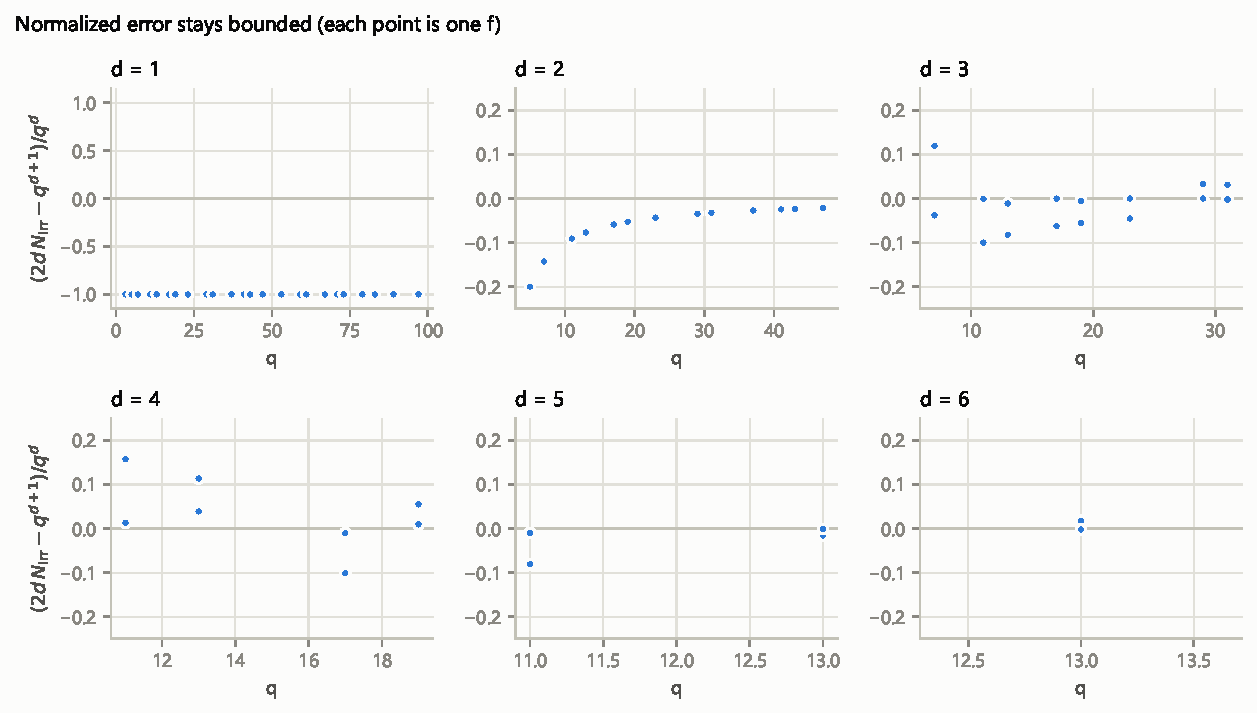
\includegraphics[width=0.9\linewidth]{../figures/fig2_normalized_error.pdf}
\caption{Normalized error $(2d\,\Nirr-q^{d+1})/q^{d}$ against $q$, for $p>2d$.
The values stay bounded, as Theorem~C requires. For $d=1$ the error is exactly $-q$.
For $d=2,3$ the values tend to $0$, in line with the $O(q^{(d+1)/2})$ error of Theorem~D.}
\label{fig:error}
\end{figure}

\subsection{The twisted identity}
For $d\le4$ and small $p$ we enumerated all of $\mathbb{F}_{p^{2d}}$ and counted
$\#W(\Fq)$ and $E(f)$ directly. The identity of Theorem~B held in every case.
$|\#W(\Fq)-q^{d+1}|$ was always far below the Cafure--Matera bound
(\texttt{data/twisted\_identity.csv}).

\subsection{Factorization statistics}
By Theorem~A and Chebotarev, the proportion of $\ba$ for which $F(t,\ba)$ has factorization
type $\lambda$ tends to $P(\lambda)=1/z_\lambda$. Figure~\ref{fig:cheb} compares the observed
frequencies with $P(\lambda)$ for $(d,p)=(2,47),(3,31),(4,19),(5,13),(6,13)$.

\begin{figure}[ht]
\centering
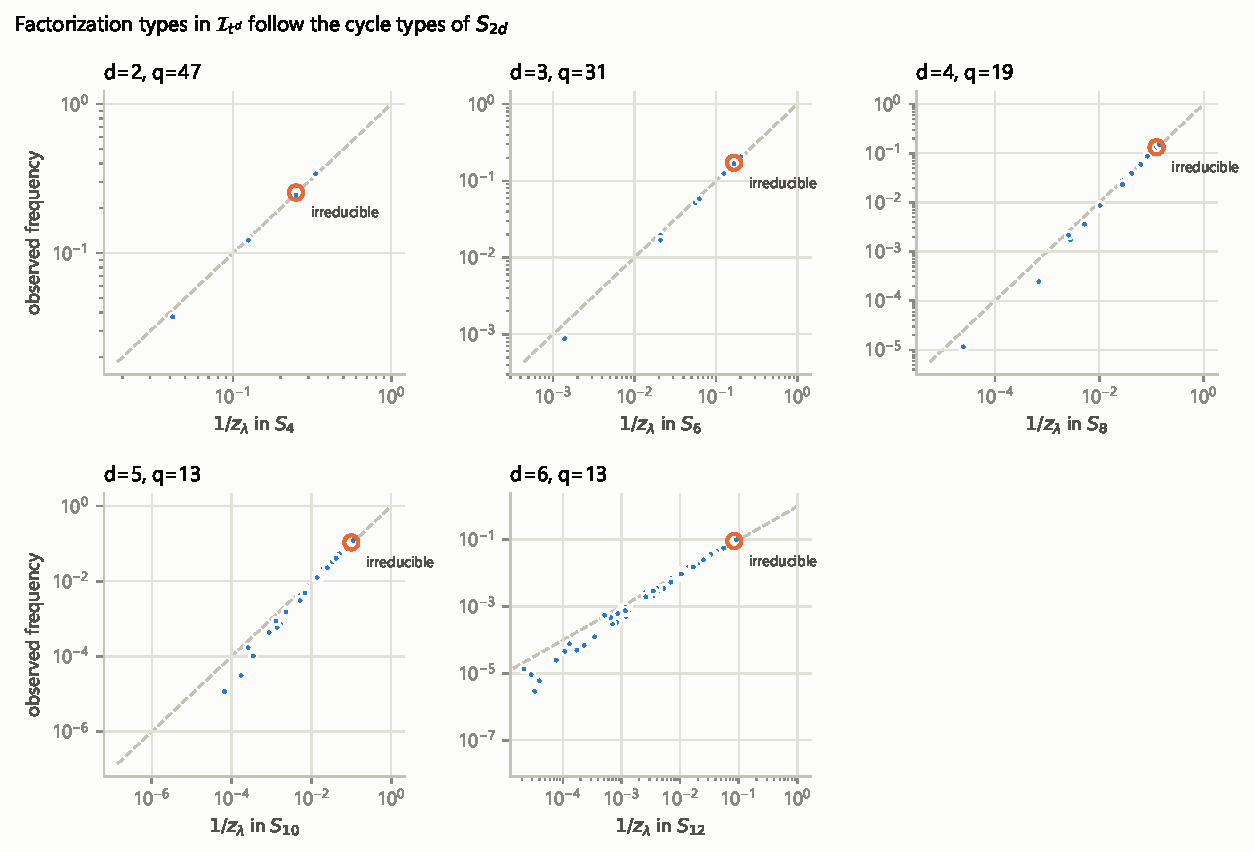
\includegraphics[width=\linewidth]{../figures/fig3_factorization_types.pdf}
\caption{Observed frequency of each factorization type in $\cI_{t^d}$ against the $S_{2d}$
cycle-type probability $1/z_\lambda$. The ringed point is the irreducible type. Points lie near the
diagonal, as full $S_{2d}$ monodromy predicts. The rarest types, with many small factors, fall below it
at these small $q$; this is the $O(q^{-1/2})$ correction.}
\label{fig:cheb}
\end{figure}

\subsection{Exhaustive search over $f$}
For small $p$ we ran over every class of $f$, using translation $t\mapsto t+b$ to set
$c_{d-1}=0$ when $p\nmid d$. Table~\ref{tab:exhaustive} gives the minimum of $\Nirr$.
It is positive in every case, including small characteristics $p\le 2d$, which are outside
Theorems~A and~C.

\begin{table}[ht]
\centering\small
\begin{tabular}{rrcrrrr}
\toprule
$d$ & $q$ & $p>2d$ & classes of $f$ & $\min N_{\rm irr}$ & $\max N_{\rm irr}$ & $q^{d+1}/2d$ \\
\midrule
2 & 3 & no & 1 & 6 & 6 & 6.8 \\
2 & 5 & yes & 1 & 30 & 30 & 31.2 \\
2 & 7 & yes & 1 & 84 & 84 & 85.8 \\
2 & 11 & yes & 1 & 330 & 330 & 332.8 \\
2 & 13 & yes & 1 & 546 & 546 & 549.2 \\
\addlinespace
3 & 3 & no & 9 & 11 & 15 & 13.5 \\
3 & 5 & no & 5 & 99 & 107 & 104.2 \\
3 & 7 & yes & 7 & 391 & 407 & 400.2 \\
3 & 11 & yes & 11 & 2418 & 2458 & 2440.2 \\
3 & 13 & yes & 13 & 4730 & 4786 & 4760.2 \\
\addlinespace
4 & 3 & no & 9 & 27 & 37 & 30.4 \\
4 & 5 & no & 25 & 375 & 402 & 390.6 \\
4 & 7 & no & 49 & 2058 & 2131 & 2100.9 \\
4 & 11 & yes & 121 & 20035 & 20420 & 20131.4 \\
4 & 13 & yes & 169 & 46212 & 46818 & 46411.6 \\
\addlinespace
5 & 3 & no & 27 & 63 & 79 & 72.9 \\
5 & 5 & no & 625 & 1450 & 1650 & 1562.5 \\
5 & 7 & no & 343 & 11654 & 11893 & 11764.9 \\
\addlinespace
6 & 3 & no & 243 & 156 & 204 & 182.2 \\
6 & 5 & no & 625 & 6383 & 6629 & 6510.4 \\
\bottomrule
\end{tabular}
\caption{Minimum and maximum of $\Nirr(f)$ over all $f$, for small $p$.
Source: \texttt{data/exhaustive\_min\_counts.csv}.}
\label{tab:exhaustive}
\end{table}

% =====================================================================
\section{Discussion}\label{sec:discussion}
% =====================================================================

\paragraph{Large $q$ versus large $d$.}
Theorems~A--D concern fixed $d$ and growing $q$. This is the regime where the
Riemann hypothesis for varieties over finite fields gives square-root cancellation.
The closer analogue of the classical conjecture fixes $q$ and lets $d\to\infty$.
That requires an irreducible polynomial of degree $2d$ with its top $d-1$ coefficients prescribed.
Known results on prescribed coefficients \cite{Pollack2013,Ha2016} allow roughly $n/4$
prescribed coefficients in degree $n$ for large $q$, and a small positive proportion for every $q$.
Half of the coefficients is out of reach of current methods, so we make no claim there.

\paragraph{Small characteristic.}
For $p\le2d$ the proofs of Propositions~\ref{prop:primitive} and~\ref{prop:transposition}
do not apply as written. By \cite{BBR2015} the asymptotic still holds for odd $p$.
Theorem~D(ii) covers $p=3$, $d=2$. The data of Table~\ref{tab:exhaustive} show no failure.

\paragraph{Open problems.}
\begin{enumerate}[label=(\arabic*),nosep]
\item Prove $\Nirr(f)\ge1$ for all $q$ when $d\ge4$, closing the gap between the
      computations (small $q$) and Corollary~\ref{cor:threshold} (large $q$).
\item Find an explicit threshold of the form $q>C^{d\log d}$ or better, using Betti-number bounds for $W$.
\item Shorter intervals: find the least $e$ such that $\{f^2+s:\deg s\le e\}$ contains an
      irreducible for all large $q$. By \cite{BBR2015} the answer is $1$ or $2$ for large $q$,
      so the real question is uniformity in $q$ and $d$.
\item Higher powers: the interval $\{f^k+s:\deg s\le(k-1)d\}$ for $k\ge3$.
\end{enumerate}

\appendix
% =====================================================================
\section{Errata to version v5}\label{app:errata}
% =====================================================================
\begin{enumerate}[label=E\arabic*.,leftmargin=*]
\item \textbf{Novelty.} The main theorem of v5, $\Nirr=q^{d+1}/(2d)+O_d(q^{d+1/2})$, is the case
      $k=2d$, $m=d$ of \cite[Thm.~2.3]{BBR2015}. That theorem also holds without the squarefree
      hypothesis and for every odd $p$. v5 cited \cite{BBR2015} only as a possible source of sharper bounds.
\item \textbf{Primitivity.} v5 used the equivalence ``imprimitive $\Leftrightarrow$ $F=g\circ h$'' for the
      Galois group of $F$ over $\Fqbar(\ba)$. That equivalence holds for $G(t)-x$ with $x$
      transcendental and appearing only in the constant term, not for a general polynomial over a field.
      The final dimension count also treated the coefficients of $g$, which lie in an algebraic
      extension of $\Fqbar(\ba)$, as free parameters in $\A^n$. Fixed in
      Lemma~\ref{lem:luroth} and Proposition~\ref{prop:primitive}.
\item \textbf{Transposition.} v5 claimed that near $\ba=0$ the discriminant has branches
      $\{P(\alpha_j)=0\}$ along which two roots coalesce. This ignores the linear term
      $P'(\alpha_j)u$ and the parameter $a_d$. When $P(\alpha_j)=0$ but $P'(\alpha_j)\ne0$, the
      double root splits. The appeal to Picard--Lefschetz was not justified in characteristic $p$.
      The remark that $p>2d$ is needed for $f'(\alpha_j)\ne0$ is also wrong, since squarefree suffices.
      Fixed in Proposition~\ref{prop:transposition}, which does not need $f$ squarefree.
\item \textbf{Effective Chebotarev.} The bound was stated with the permutation sheaf $\pi_*\overline{\mathbb Q}_\ell$.
      Traces of Frobenius on that sheaf count fixed points, so they detect linear factors,
      not $2d$-cycles. Counting $2d$-cycles needs all irreducible characters of $S_{2d}$ that are
      nonzero on the class, which are the $2d$ hook characters. The cited
      ``\cite{Katz1988}, Thm.~9.2.6'' is not an effective Chebotarev theorem. Replaced by Theorem~B.
\item \textbf{Betti-number bound.} v5 attributed $B(\mathcal F)\le N(2\delta+1)^n$ to
      \cite[Thm.~12]{Katz2001}. That theorem bounds Betti numbers of Artin--Schreier and Kummer
      sheaves $\mathcal L_\psi(f)\otimes\mathcal L_\rho(G)$, not of push-forwards of finite covers.
      The general bounds for compatible systems in \cite{Katz2001} are not explicit.
      So the threshold $(8d)^{2d+6}$ was unproved. Replaced by Corollary~\ref{cor:threshold}.
\item \textbf{Error term bookkeeping.} In Step 4 of v5 the unspecified $O_{N,n}(q^{n-1})$ term of the
      Chebotarev bound was replaced by a Lang--Weil count of $\mathcal D(\Fq)$. These are different
      quantities, and the latter is not needed because $\Nirr=\Nirr^\circ$.
\item \textbf{GOS formula.} Equation (4.1) of v5 wrote $\chi(\mathbb P^1,j_!\mathcal F)=2r-\sum(\mathrm{drop}_v+\mathrm{Sw}_v)$.
      That is the formula for $j_*$, not $j_!$. The section was not used in the proof and is omitted.
\item \textbf{Citations.} Bary-Soroker's paper is \emph{Proc.\ AMS} 137 (2009), 73--83, not vol.\ 140 (2012),
      and it works over PAC fields rather than via Chebotarev over finite fields.
      Several bibliography entries were never cited.
      The Arnold--Gusein-Zade--Varchenko reference was dated inconsistently.
\item \textbf{Numerical evidence.} v5 inferred that $\Nirr\ge1$ ``for all $q$ and $d$'' from three small
      examples. Section~\ref{sec:numerical} replaces them with systematic data. The general claim
      remains open for $d\ge4$.
\item \textbf{Version-history remarks} in the body of v5 (``erroneously used in earlier versions'')
      have been moved to this appendix.
\end{enumerate}

\begin{thebibliography}{99}

\bibitem{BHP2001}
R.\,C.~Baker, G.~Harman, J.~Pintz,
The difference between consecutive primes, II,
\textit{Proc.\ London Math.\ Soc.}\ \textbf{83} (2001), 532--562.

\bibitem{BBR2015}
E.~Bank, L.~Bary-Soroker, L.~Rosenzweig,
Prime polynomials in short intervals and in arithmetic progressions,
\textit{Duke Math.\ J.}\ \textbf{164} (2015), 277--295. arXiv:1302.0625.

\bibitem{BS2009}
L.~Bary-Soroker,
Dirichlet's theorem for polynomial rings,
\textit{Proc.\ Amer.\ Math.\ Soc.}\ \textbf{137} (2009), 73--83.

\bibitem{CM2006}
A.~Cafure, G.~Matera,
Improved explicit estimates on the number of solutions of equations over a finite field,
\textit{Finite Fields Appl.}\ \textbf{12} (2006), 155--185. arXiv:math/0405302.

\bibitem{Carlitz1952}
L.~Carlitz,
A theorem of Dickson on irreducible polynomials,
\textit{Proc.\ Amer.\ Math.\ Soc.}\ \textbf{3} (1952), 693--700.

\bibitem{ChenV5}
R.~Chen,
The geometry of prime vacuums: Legendre's conjecture in function fields via monodromy and
Chebotarev density (v5), Zenodo, 2026. \url{https://doi.org/10.5281/zenodo.18705744}

\bibitem{Deligne1980}
P.~Deligne,
La conjecture de Weil.~II,
\textit{Publ.\ Math.\ IH\'ES} \textbf{52} (1980), 137--252.

\bibitem{DM1996}
J.\,D.~Dixon, B.~Mortimer,
\textit{Permutation Groups}, GTM 163, Springer, 1996.

\bibitem{Fulton1998}
W.~Fulton,
\textit{Intersection Theory}, 2nd ed., Springer, 1998.

\bibitem{Ha2016}
J.~Ha,
Irreducible polynomials with several prescribed coefficients,
arXiv:1601.06867, 2016.

\bibitem{Katz1988}
N.\,M.~Katz,
\textit{Gauss Sums, Kloosterman Sums, and Monodromy Groups},
Ann.\ of Math.\ Stud.\ 116, Princeton Univ.\ Press, 1988.

\bibitem{Katz2001}
N.\,M.~Katz,
Sums of Betti numbers in arbitrary characteristic,
\textit{Finite Fields Appl.}\ \textbf{7} (2001), 29--44.

\bibitem{LL2016}
M.~Lal\'in, O.~Larocque,
The number of irreducible polynomials with the first two prescribed coefficients over a finite field,
\textit{Rocky Mountain J.\ Math.}\ \textbf{46} (2016), 1587--1618.

\bibitem{LN1997}
R.~Lidl, H.~Niederreiter,
\textit{Finite Fields}, 2nd ed., Encyclopedia Math.\ Appl.\ 20, Cambridge Univ.\ Press, 1997.

\bibitem{MY2016}
G.~McGuire, E.\,S.~Y\i lmaz,
The number of irreducible polynomials with the first two coefficients fixed over finite fields of
odd characteristic, arXiv:1609.02314.

\bibitem{Muller1995}
P.~M\"uller,
Primitive monodromy groups of polynomials, in
\textit{Recent Developments in the Inverse Galois Problem}, Contemp.\ Math.\ \textbf{186},
Amer.\ Math.\ Soc., 1995, 385--401.

\bibitem{Pollack2013}
P.~Pollack,
Irreducible polynomials with several prescribed coefficients,
\textit{Finite Fields Appl.}\ \textbf{22} (2013), 70--78.

\bibitem{Turnwald1995}
G.~Turnwald,
On Schur's conjecture,
\textit{J.\ Austral.\ Math.\ Soc.\ Ser.~A} \textbf{58} (1995), 312--357.

\end{thebibliography}
\end{document}
